\chapter{Alkalmazás migrálása a Docker Compose-ból a Kubernetesbe}

\section{Bevezetés}

A konténerizáció nagy előnyt nyújt, mivel szabványosított, elszigetelt környezetet kínál a szoftverek futtatásához. 
A Docker Compose elterjedt a helyi, több konténert tartalmazó alkalmazásokhoz, egyszerűsítve az összekapcsolt 
szolgáltatások definiálását és futtatását. Mivel azonban sokszor skálázódásra van szükség, és olyan funkciókra, 
mint a nagy rendelkezésre állás, az automatikus skálázás és a kifinomult orkesztráció, a Kubernetes vált a konténer 
orkesztráció szabványává.

Ebben a fejezetben megmutatom, hogy az eredetileg a Docker Compose segítségével definiált rendszeremet, 
hogyan migráltam Kubernetes környezetbe. A rendszeremben a már meglévő szolgáltatások jelenek meg, mint a 
Prometheus a felügyelethez, a Grafana a vizualizációhoz, több szimulátorszolgáltatás és egy vezérlőszerver. 
Itt bemutatom a Docker Compose konfigurációk Kubernetes manifesztekbe való átforgatásának kihívásait.

\section{A Docker Compose és Kubernetes áttekintése}

Docker Compose
Ezzel több konténert tartalmazó Docker alkalmazásokat lehet definiálni és futtatni. 
Konfigurációja egy YML fájlban tárolt, ahol a szolgáltatásokat, hálózatokati kapcsolatokat, köteteket és 
függőségeket lehet megadni. A Docker Compose leegyszerűsíti a konténerek egyetlen hoszton történő orkesztrációját, 
így segíti a fejlesztést és tesztelést.

Kubernetes
A Kubernetes viszont egy robusztus, open source platform a konténerek telepítésének, 
skálázásának és üzemeltetésének automatizálására hostokon. A Kubernetes új absztrakciókat vezet be:

\begin{itemize}
    \item Pod: Ez a legkisebb telepíthető egység, amely egy vagy több konténert foglalnak magukba.
    
    \item Deployment: Állapot nélküli alkalmazások kezelésére szolgáló objektumok, amelyek olyan funkciókat kínálnak, mint a gördülő frissítések és a visszaállítás.
    
    \item Service: Végpontokat biztosítanak a podok eléréséhez, segítve a felfedezést és a terheléselosztást.
    
    \item ConfigMap és Secret: Mechanizmus a konfiguráció és az imagek szétválasztására.
    
    \item PersistentVolumeClaim (PVC): Absztrakció adattárolásra.
\end{itemize}

A migráció során ezeket képeztem le docker-ből k8-ba.

\begin{figure}[!ht]
    \centering
    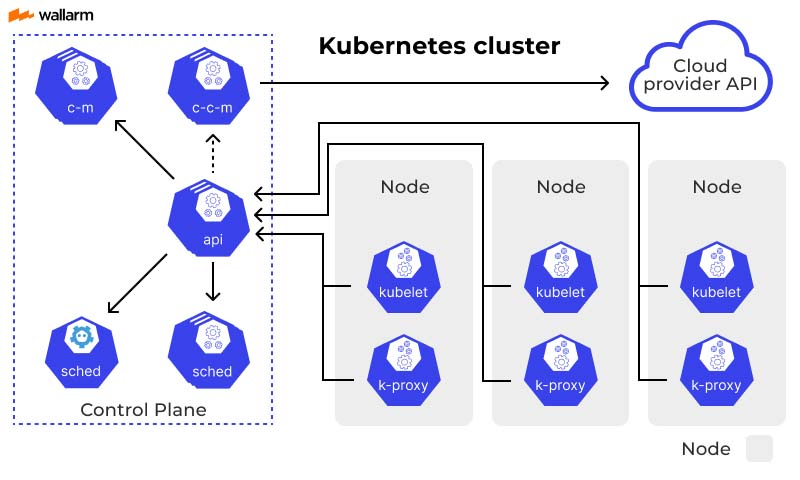
\includegraphics[width=0.8\textwidth, keepaspectratio]{figures/components-of-kubernetes.jpeg}
    \caption{Kubernetes architektúra \cite{wallarm_kubernetes_cluster}} 
\end{figure}

\section{Rendszerarchitektúrája}

A rendszer a már megismert következő részeket tartalmazza:

\begin{itemize}
    \item Prometheus: Egyéni prometheus.yml fájllal konfigurált idősoros adatbázis. 
    Ennek szerencsétlensége, hogy az újra konfiguráció csak újra indítással lehetséges.
    
    \item Grafana: Vizualizációs eszköz, ami közvetlen a Prometheushoz kapcsolódik megjelenítéséhez.
    
    \item ESP8266 szimulátorok: Itt épen három példány szimulálja a különböző szimulátorazonosítókkal 
    rendelkező eszközöket.
    
    \item Breaker Simulators: Más jellegű, de hasonló célú szimulátor.
    
    \item Vezérlőszerver: Lebonyolítja az eszközök közötti interakciókat, vezérlést és adatok továbbítását.
    
    \item System Simulator: A rendszer általános viselkedését emuláló központi szolgáltatás.
\end{itemize}

A Docker Compose alkalmazásban ezek az összetevők hálózaton és socketeken keresztül kapcsolódtak össze, 
és meghatározott végpontokon jelenítettek meg. \cite{docker_kubernetes}

\section{A Docker Compose beállítások konvertálása Kubernetes manifesztekké}

A Docker Compose-ról a Kubernetesre való áttérés magában foglalja az alkalmazás architektúrájának 
újragondolását a podok, deployement-ek, szolgáltatások és más Kubernetes objektumok szerint. \cite{kubernetes}

\subsection{Névtér- és konfigurációkezelés}

Itt létrehoztam egy névteret (pl. monitoring) ez izolációt biztosít az alkalmazás számára. 
A ConfigMap a Prometheus konfiguráció tárolására szolgál (a prometheus.yml tartalma), 
lehetővé téve a konfiguráció frissítését a konténerek image-einek újbóli legenerálása nélkül.

\begin{lstlisting}
    apiVersion: v1
kind: Namespace
metadata:
  name: monitoring
---
apiVersion: v1
kind: ConfigMap
metadata:
  name: prometheus-config
  namespace: monitoring
data:
  prometheus.yml: |-
    global:
      scrape_interval: 15s
    scrape_configs:
      - job_name: 'prometheus'
        static_configs:
          - targets: ['localhost:9090']
\end{lstlisting}

\subsection{Deployment-ek és Service-ek}

Minden szolgáltatás Docker Compose-ban egy Deployment és egy Service formájában jelenik meg a Kubernetesben. 
A Deployment kezeli az alkalmazásban a podokat, a Service ezeket a podokat teszi elérhetővé.

Például a Prometheus szolgáltatás egyetlen replikával rendelkezik. Konfigurációja a ConfigMap-ról van mountolva, 
a perzisztens adatai pedig egy PersistentVolumeClaim (PVC) segítségével tárolom. Hasonlóképpen, más szolgáltatások, 
például az ESP8266 szimulátorok és a vezérlő szerver deployement-ekké alakulnak át, amelyek környezeti változókat 
és portkonfigurációkat adnak meg.

\subsection{Perzisztens tárolók kezelése}

A Docker Compose-ban gyakran definiálnak volume-okat az adattárolására. A Kubernetesben ezt a 
PersistentVolumeClaims biztosítja. A készített rendszeremben a Prometheus, mind a Grafana perzisztens 
tárolót igényelt az adatok megőrzéséhez, amiket a PVC-k létrehozásával és konténerekhez kötésével értem el.

\begin{lstlisting}
  apiVersion: v1
kind: PersistentVolumeClaim
metadata:
  name: grafana-data
  namespace: monitoring
spec:
  accessModes:
    - ReadWriteOnce
  resources:
    requests:
      storage: 1Gi
\end{lstlisting}

\subsection{Szolgáltatások elérhetővé tétele és hálózati konfiguráció}

A Docker Compose-ban a portok hozzárendelését a konfigurációban végezzük. 
A Kubernetesben a portok meghatározást a Service-ek kezelik, ezek lehetnek 
NodePort típusúak a külső hozzáféréshez vagy ClusterIP típusúak a belső kommunikációhoz. 
A migráció során a konténerek portjait le kellett képezni a hosztokra, hogy a külső interfész 
ugyanaz maradjon az eredeti Docker Compose-hoz képest.

Például a Docker Compose-ban az 5000-es porton található vezérlő szervert egy olyan Kubernetes Service replikálja, 
amely egy adott NodePort-ot rendel hozzá, például 30050-et.

\subsection{Telepítés és tesztelés}

A Kubernetes manifeszt a kubectl apply -f paranccsal kerül alkalmazásra. Ez telepíti az összes komponenst a névtérben. 
A telepítés után a szabványos Kubernetes-parancsok (pl. kubectl get pods, kubectl logs, kubectl describe) 
a podok állapotának ellenőrzésére szolgálnak. Így iteratívan lehet tesztelni az új rendszert és később 
szolgáltatás kimaradás nélkül frissíteni.

Telepítéséhez a következő parancsot használjuk:

\begin{lstlisting}
  kubectl apply -f monitoring.yaml
\end{lstlisting}

És hogy megvizsgáljuk a telepített podokat:

\begin{lstlisting}
  kubectl get pods -n monitoring
\end{lstlisting}
